\chapter{Results}

\section{The article}

\subsection{Never scanned area}

In this tableau below, we can see the results about the percentage of the map never scanned.\\\\

\begin{tabular}{|c|c|c|c|}
\hline
	      & Max & Median & Min \\
	      \hline
	Random & 16.2\% & 3.2\% & 0.5\% \\
	\hline
	Pheromone & 0.21\% & 0.03\% & 0.01\% \\
	\hline
\end{tabular}
\\\\
It represents  the maximum, median and minimum uncovered area for the ten runs.These numbers  clearly  show  the  ability  of  the  pheromone 
model to cover the complete area. 

\subsection{Connectivity}

\begin{figure}[h]
\caption{\label{randomconnect} Random. Number of UAVs in contact with C\&C (max, average, min)}
   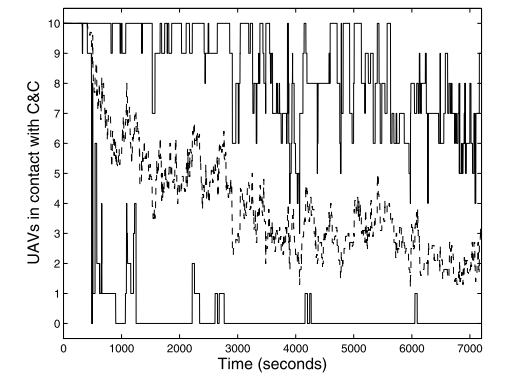
\includegraphics{../images/random_resultat_connectivite.png}
\end{figure}

\begin{figure}[h]
\caption{\label{pheromoneconnect}Pheromone. Number of UAVs in contact with C\&C (max, average, min)}
   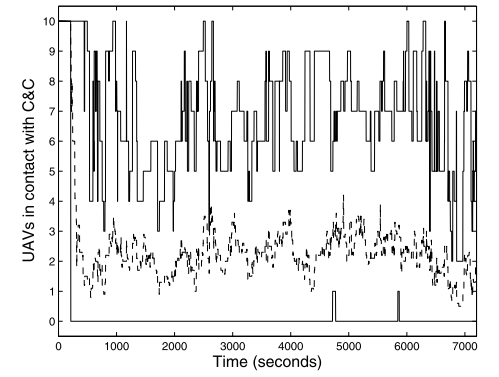
\includegraphics{../images/pheromone_resultat_connectivite.png}
\end{figure}
In Figure \ref{randomconnect} and Figure \ref{pheromoneconnect}...